%!TEX TS-program = xelatex
\documentclass[]{friggeri-cv}

\usepackage{afterpage}
\usepackage{xeCJK}
%\usepackage[slantfont, boldfont]{xeCJK}
\usepackage{hyperref}
\usepackage{color}
\usepackage{xcolor}
\definecolor{myblue}{RGB}{4, 98, 249}
\usepackage{hyperref}
\hypersetup{
    pdftitle={},
    pdfauthor={},
    pdfsubject={},
    pdfkeywords={},
    colorlinks=true,       % no lik border color
    allbordercolors=white    % white border color for all
}
\addbibresource{bibliography.bib}
\RequirePackage{xcolor}
\definecolor{pblue}{HTML}{0395DE}


% ------------
\usepackage{enumitem}
\renewenvironment{entrylist}{%
  \begin{itemize}[leftmargin=1in]%[leftmargin=*,align=left,itemindent=-\dimexpr\labelwidth+\labelindent+\labelsep\relax]
  }{%
  \end{itemize}
}
\renewcommand{\bfseries}{\headingfont\color{headercolor}}
\renewcommand{\entry}[4]{%
\item[#1]
  \textbf{#2}%
  \hfill%
  {\footnotesize\addfontfeature{Color=myblue} #3}\\%
  #4\vspace{\parsep}%
}
% -------


\begin{document}


\header{闫}{博阳}


% Fake text to add separator      
\fcolorbox{white}{gray}{\parbox{\dimexpr\textwidth-2\fboxsep-2\fboxrule}{%
.....
}}

% In the aside, each new line forces a line break
\begin{aside}
  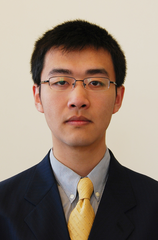
\includegraphics[scale=0.07]{img/boyang.png}
  \section{地址}
  天津市南开区宾水西
  道华苑新城竹华里
    ~
    \section{联系方式}
    \textbf{电话号码:} +86 18512290791
    \textbf{Skype:} yanboyang
    \textbf{微信:} yanboyang713
    ~
    \section{邮箱}
    \href{mailto:by932@uowmail.edu.au}{\textbf{by932@}\\uowmail.edu.au}
    \href{mailto:yanboyang713@gmail.com}{\textbf{yanboyang713@}\\gmail.com}
    ~
    \section{个人主页及Github}
    \href{https://github.com/yanboyang713}{github.com/yanboyang713}
    \href{http://www.yanboyang.com}{yanboyang.com}
    ~
    \section{程序语言}
    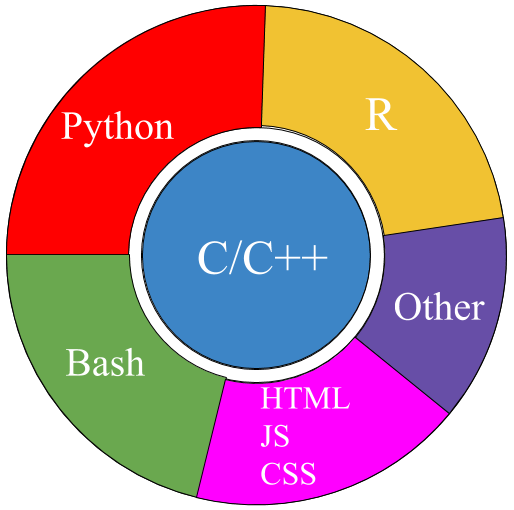
\includegraphics[scale=0.2]{img/programming.png}
    ~
    \section{OS 偏好}
    \textbf{GNU/Linux}
\includegraphics[scale=0.40]{img/5stars.png}
    \textbf{Unix}
\includegraphics[scale=0.40]{img/4stars.png}
    \textbf{MacOS}
\includegraphics[scale=0.40]{img/3stars.png}
    \textbf{Windows}
\includegraphics[scale=0.40]{img/1stars.png}
    ~
\end{aside}



% \section{Person Statement}


本人科研探索能力较强,现发表有一篇论文(关于机器翻译质量测试),现正在书写一篇文
本不同性验证专利及一篇关于机器翻译与感情倾向分析相结合的文章。在学校期间,得过优
秀学生奖学金及获得最佳毕业设计。一共参加过两次国际学术会议。知识较为全面,热衷于技术。
\section{工作经历}
\begin{entrylist}
  \entry
  {2018.12 至今\\}
  {\large{算法工程师}}
  {鹏城实验室, 深圳, 中国}
  {主要工作内容:\\\\
    3d打印小型无人机\\
    小型无人机硬件系统的构建\\
    飞控系统仿真平台\\
    完善文本不同性验证系统,先发专利,后发文章。\\
    完善机器翻译质量测量系统,及发paper\\
    制定实验室测试标准\\
    软件定义网络更新策略的研究结合蜕变测试\\
    探索3d打印切片工具的测试\\}

\end{entrylist}

\section{教育背景}
\begin{entrylist}

  \entry
    {2018.1 - 2018.11\\}
    {\large{ 研究硕士 (计算机科学)}\\}
    { 伍伦贡大学(澳大利亚)}
    {Metamorphic Testing (软件测试方向)\\
      \textbf{主要课程}: 软件测试, 研究方法, 大数据分析, 自然语言处理\\
      \textbf{主要成果}: \underline{发表一篇文章,有关机器翻译}\\
      Metamorphic Relations for Data Validation: A Case Study of Translated Text Messages}

  \entry
    {2014.3 - 2017.12\\}
    {\large{计算机科学本科}​}
    {伍伦贡大学(澳大利亚)}
    {方向软件工程\\\\
      \textbf{主要课程}:\\
      算法与数据结构(80 优秀)\\
      面向对象编程C++ (75 优秀)\\
      交互式计算机图形 (75 优秀)\\
      多媒体 (73 )\\
      软件工程练习及规范 (82 优秀)\\\\
      \textbf{主要成果}:\\
      1. 毕业最佳项目 ({\footnotesize 刷卡系统})\\
      2. 本科优秀学生奖学金\\
    }
  \entry
  {2013.3 - 2014.3}
  {\large{学术英语}}
  {伍伦贡大学(澳大利亚)}
  {}

  \entry
    {2011.9 - 2013.3\\}
    {\large{工商管理(本科)}\\}
    {中国矿业大学}
    {平均分 91\% \\
      \textbf{主要课程}: \\高等数学1:满分,高等数学2:84}

\end{entrylist}

\newpage

\section{发表文章}
Boyang Yan, Brian Yecies, Zhi Quan Zhou: Metamorphic Relations for Data
Validation: A Case Study of Translated Text Messages. IEEE/ACM 4th International
Workshop on Metamorphic Testing (MET '19), in conjunction with the 41st
International Conference on Software Engineering (ICSE '19), Montreal, Canada;
05/2019

\section{学术会议}
\begin{entrylist}
  \entry
  {5月26日, 2019}
  {\\论文报告 - 题目:\\ Metamorphic Relations for Data Validation:\\
    A Case Study of Translated Text Messages}
  {ICSE, 蒙特利尔, 加拿大}

  \entry
  {8月11日, 2017}
  {展示毕业项目 - 刷卡系统(硬件原型及软件)\\}
  {IEEE Sections Congress (SC2017), 悉尼,澳大利亚}

\end{entrylist}

\section{证书及获奖}
\begin{entrylist}
  \entry
    {2017}
    {澳大利亚业余无线电操作证(标准)\\}
    {澳大利亚无线电协会(WIA)}

  \entry
    {2016}
    {Ross a. Hull memorial Vhf-Uhf  无线电比赛\\}
    {澳大利亚无线电协会(WIA)}
    {12 名 Section A (模拟模式, 最好 7 天) 及 Section C (模拟模式, 最好两天)}

  \entry
    {2014}
    {澳大利亚业余无线电操作证(基础)\\}
    {澳大利亚无线电协会(WIA)}
   
  \entry
    {2010}
    { 天津市第 92 届中小学运动会篮球第 2 名\\}
    {Tianjin Basketball Tryouts, China}
    {高中男子 B 组及篮球 2 级运动员证}

\end{entrylist}

\section{培训课程}
\begin{entrylist}
  \entry
  {18.11.2018}
  {Sololearn(C++)}
  {Sololearn}

  \entry
  {2.9.2017}
  {Sololearn(Python3)}
  {Sololearn}

  \entry
    {2012}
    {Intel innovation in EDUCATION}
    {Intel Learn Program (Technical and Community)}

  \end{entrylist}

\begin{aside}
  \section{语言}
  \textbf{中文}
\includegraphics[scale=0.40]{img/5stars.png}
  \textbf{英语}
\includegraphics[scale=0.40]{img/4stars.png}
\end{aside}


\newpage

\section{业余活动}
我最主要的业余活动是业余无线电(amateur radio)。在 2014 年,考取了第一个业余
无线电操作证 (foundation license)。刚开始只是为了练习英语通过与世界各地无线电爱
好者交流。之后,目的慢慢开始变化,因为我发现业余无线电与计算机十分有联系,特
别是数字模式。比如 SSTV 可以用于传输图片,D-STAR 数字模式可以传输数据及数字
语音。甚至国际空间站也有也有业余无线电中继站。从练习英语慢慢变成了关注研究业
余无线电的技术部分,比如天线的结构,数字模式等。同时也参加一些业余无线电比赛
并在澳大利亚 ross a. Hull memorial vhf-uhf 比赛中获得名次。

\section{ 学校项目}
\begin{entrylist}
  \entry
    {2017}
    {使用OPENGL模拟创建一间房间\\}
    {伍伦贡大学(澳大利亚)}
    {使用OPENGL模拟创建了一间房间包括墙壁,地板,2幅画,桌椅及灯光等}
\end{entrylist}

\begin{entrylist}
  \entry
    {2017}
    {OPENGL 行星运动系统\\}
    {伍伦贡大学(澳大利亚)}
    {使用OPENGL建立了一个行星运动系统
    \\\\ Github链接: \\{\small\url{https://github.com/yanboyang713/openGLPlanetarySystem.git}}}
\end{entrylist}

\begin{entrylist}
  \entry
    {2016}
    {5th order低通Butterworth滤波器\\}
    {伍伦贡大学(澳大利亚)}
    {使用SDL库编写了一个5th order低通Butterworth滤波器,用于处理声音已减少噪音。
     \\\\ Github链接: \\{\small\url{https://github.com/yanboyang713/butterworthFilter.git}}}
\end{entrylist}

\begin{entrylist}
  \entry
    {2016}
    {编写直方图均衡和灰度变换增强算法\\}
    {伍伦贡大学(澳大利亚)}
    {使用SDL编写直方图均衡和灰度变换增强算法,加强对比度和显示图片。
     \\\\ Github链接: \\{\small\url{https://github.com/yanboyang713/histogramEqualizationImage.git}}}
\end{entrylist}

\begin{entrylist}
  \entry
    {2017}
    {Tries数据结构\\}
    {伍伦贡大学(澳大利亚)}
    {使用Tries数据结构,用于文章词频统计,并排序。
     \\\\ Github链接: \\{\small\url{https://github.com/yanboyang713/tries-data-structure-count-unique-word-frequency.git}}}
\end{entrylist}

\begin{entrylist}
  \entry
    {2017}
    {商店服务模拟\\}
    {伍伦贡大学(澳大利亚)}
    {商店服务模拟drive by event 而不是 by time,主要使用了heap及queue。
     \\\\ Github Link: \\{\small\url{https://github.com/yanboyang713/simulate-shop-service.git}}}
\end{entrylist}

\begin{entrylist}
  \entry
    {2017}
    {彩虹表\\}
    {伍伦贡大学(澳大利亚)}
    {使用c++编写彩虹表用于破解哈希算法。
    \\\\ Github链接: \\{\small\url{https://github.com/yanboyang713/rainbowTable.git}}}
\end{entrylist}

\begin{entrylist}
  \entry
    {2017}
    {刷卡系统\\}
    {伍伦贡大学(澳大利亚)}
    {使用Arduino, 树莓派, level shifter, LCD 控制器和 LCD 显示器制作考勤刷卡系统。在树莓派中,编写及使用Python实现树莓派与Arduino和Java后台通讯。并且使用I2C bus链接树莓派, Arduino 和 LCD控制器。使用Level shifter在I2C bus中转换不同电压。 RFID传感器与Arduino相连接。在Arduino中, 我写的c语言。}
  \end{entrylist}

\section{Referral Info}
\begin{itemize}
	\item George Zhou <zhiquan@uow.edu.au> Research Project
	\item Jack Yang <jiey@uow.edu.au> Research Project
	\item Eve Shaw <eve@uow.edu.au> English aspect
	\item Mark Freeman <mfreeman@uow.edu.au> undergraduate final project
	\item Casey Chow <caseyc@uow.edu.au> computer graphics aspect
	\item Tianbing Xia <txia@uow.edu.au> base programming aspect and database aspect
\end{itemize}











\begin{flushleft}
  \today
\end{flushleft}
\begin{flushright}
\emph{Boyang Yan}
\end{flushright}

%%% This piece of code has been commented by Karol Kozioł due to biblatex errors. 
% 
%\printbibsection{article}{article in peer-reviewed journal}
%\begin{refsection}
%  \nocite{*}
%  \printbibliography[sorting=chronological, type=inproceedings, title={international peer-reviewed conferences/proceedings}, notkeyword={france}, heading=subbibliography]
%\end{refsection}
%\begin{refsection}
%  \nocite{*}
%  \printbibliography[sorting=chronological, type=inproceedings, title={local peer-reviewed conferences/proceedings}, keyword={france}, heading=subbibliography]
%\end{refsection}
%\printbibsection{misc}{other publications}
%\printbibsection{report}{research reports}

\end{document}
